\documentclass[journal,10pt,onecolumn,compsoc]{IEEEtran} \usepackage[margin=1.0in]{geometry} \usepackage{pdfpages} 

%\usepackage{color}
\usepackage{geometry}
\usepackage{graphicx}
\usepackage{amsthm}
\usepackage{amssymb}
\usepackage{amsmath}
\usepackage{float}
\usepackage{balance}
\usepackage{enumitem}
\usepackage{pstricks, pst-node}
\usepackage{hyperref}
\usepackage{url}

\hypersetup{
  colorlinks = false,
  urlcolor = black,
  pdfkeywords = {CS461``Senior Software Engr Project''Problem Statement},
  pdftitle = {CS 461 Problem Statement},
  pdfsubject = {CS 461 Problem Statement},
  pdfpagemode = UseNone
}

\begin{document}
\begin{center}
  
  \textbf{}

  \vspace{2.5cm}
  \Huge{}
  \textbf Problem Statement
  \vspace{1.5cm}

 
  \LARGE
  CS461 - Senior Software Engr Project\\
  \vspace{0.25cm}
  Group 36: Data Interactive Visualization Application(DIVA)\\
  Instructor: D. Kevin McGrath \\
  Instructor: Kirsten Winters \\
  \vspace{0.25cm}
  Fall 2018 \\
  \vspace{1cm}
  
  \large{Matthew Jansen, Bhavya Parikh, Davian Lukman, Eli Laudi, Ryan Sisco}\\
  \vfill
  November 27th, 2018\\
  \vspace{1cm}
  \vspace*{\fill}
   \begin{abstract}
     When data is presented in a large set, sometimes it can't be easily understandable in its raw form. This paper will propose a solution to the problems of presenting new data in a meaningful and unique way in the form of a web application. We will describe the problem in depth and the implications that it has in industry and academia. Then, we will propose a detailed solution to the issue using an application to visualize data in a 3D environment, which will map not only the objects within each file but their relationships as well. Lastly, we will define performance metrics to measure the applicability and accuracy of the application.
       \noindent 
   \end{abstract}
   \normalsize 
  \end{center}
\newpage
\tableofcontents
\newpage

\section{PROBLEM DESCRIPTION}
    One recurring challenge in a variety of fields is the ability to present and visualize data in new ways, especially the case for large data sets which can be difficult to visualize, let alone find relationships or patterns in. Humans are able to interpret data sets more accurately and thoroughly when presented in the form of a visual image, compared to reading and sorting through several log files, attempting to find correlations and draw conclusions by hand.\\
    \newline
    Furthermore, given certain data-types such as IP address and their corresponding geo-locations, names and hashes of malware, and other various tags, it can be helpful to visualize these objects in a 3D environment. Without the ability to view data in this format, it can be difficult to see how objects within a data set interact with each other and define how inter networks of these objects might operate in a given context or environment. On the other hand, some researcher also argued that there are drawbacks from using 3D visualization. The drawbacks could be an over-complicated graph with less details and lack of accuracy.\\
    \newline
    Either way, not having an correct and concise data visualization could have a negative impact in both industry and academia, as it prevents a complete content from being brought forward to their respective customers and researchers. This pitfall can also have negative impacts in a time-constrained environment, such as when conducting network forensics to determine the source of unwanted malware within a network, and identifying it accordingly based off fingerprints.

\section{PROPOSED SOLUTION}
There are several open source solutions to display data in a 3D manner. However, these solutions have their own input type that the data might not come prepackaged as. Our solution is to develop a program which will consume CSV spreadsheet files, extract the data from them, and display that data in a friendly 3D manner. The initial starting point of this project is to handle data both geographically and temporally, meaning that the data is displayed both in accordance to geography and timeline to adjust the temporal history. For example, the tool will consume a CSV file that McAfee will provide us. It will contain data such as geographical, malware related, and temporal. The tool will have to parse the data and translate it into 3D coordinates as well as mapping all associated data to that point.\\
\newline
 The principle of transforming the data is simple. The complexity of this part of the application would come from the ability for the application to consume CSV files that contain differing types of information. One CSV file might contain geographical data, while another may contain spatially related data; the application would be able to handle both. This is a feature that may not be part of version one, but could very well be implemented.\\
\newline
The second part of the process is the visualization itself. The data obtained from the first part of the process will be used and mapped onto a 3D space where the application will represent the data sets with points in space or on a globe. This data will be organized spatially and use colors to denote user-desired specifications. These specifications will be supplied in the CSV file from part one. The user will be able to explore the 3D data set using click and drag.
    
    \subsection{CSV Data Input}
    There are several open source solutions to display data in a 3D manner. However, these solutions have their own input type that a lot of data might not come prepackaged as. Our solution is to come up with a program which will consume CSV spreadsheet files, extract the data from them, and display that data in a friendly 3D manner. \\
    \newline
    Data should be input from a GUI, however, for raw functionality, it can be pulled in from a command line just for the developmental purpose. There are solutions to do this in nearly every programming language, so the choice in languages comes down to a performance and preference basis, the top contenders being Java or Python. We would most likely translate the data into JSON format, allowing for hierarchical sorting with least-pertinent data nested the deepest.\\
    \newline
    The principle of transforming the data is simple. The complexity of this part of the application would come from the ability of the application to consume CSV files that contain different types of information. One CSV file might contain geographical data, while another may contain spatially related data; the application would be able to handle both. This is a feature that may not be part of version one, but could very well be implemented.\\
    \newline
    Depending on user preference, a graphical interface will be developed to make it easier to choose files and settings. If preferred, it can also allow a console to input commands directly. This all depends on how its priority to the client.\\

    \subsection{Data Population}
    This will be the most challenging part of the project. There are many open source projects that create 3D models of the earth that are able to be populated. This will take a lot of time to get running in a stable way, that works with our given data. We would also like to add extra features such as color, different 3D models, better interface, etc. This would be developed later on after the base project is done.\\

    \subsection{3D Rendering}
    After the project works with 1 3D model, we can include and create different visualizations. This is all ”filler” and can be added non-stop until the project is done. We will reach out and collaborate on renderings that are requested by everyone.\\
    \newline
    One of the most important parts of this assignment is differentiating the data. This project includes adding multiple data points such as dates and malware type. It would be a great addition to add an option to sort colored data by date or malware.\\
     
     \begin{figure}[H]
         \centering
         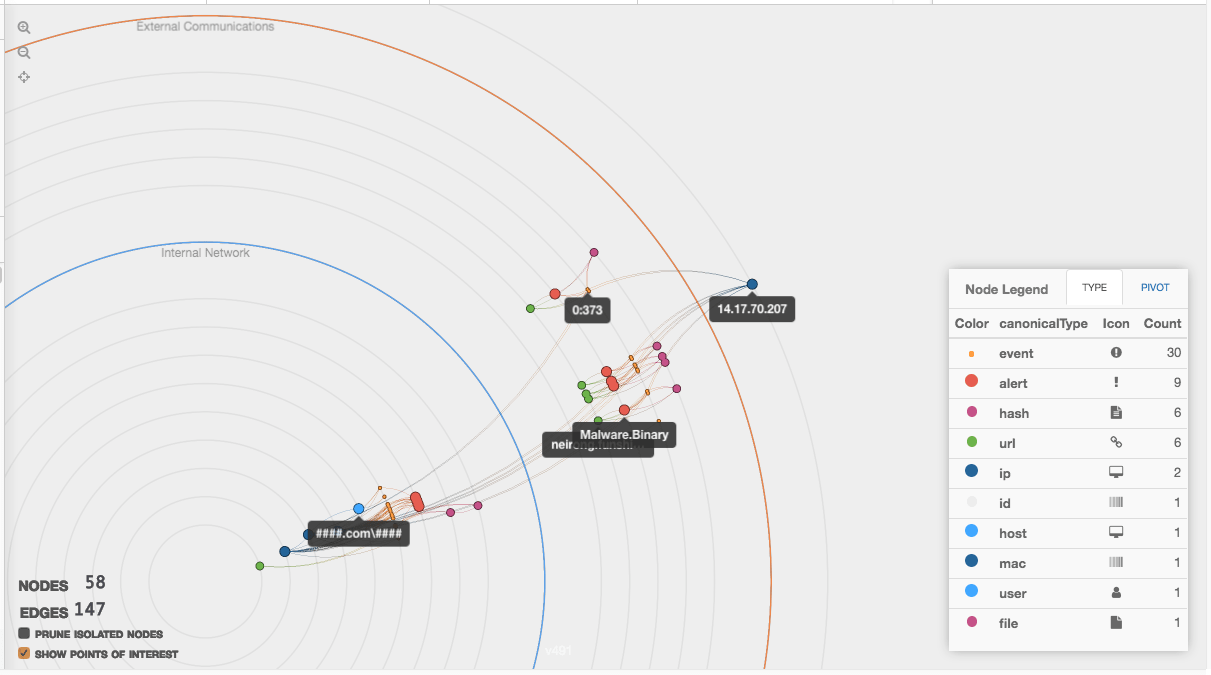
\includegraphics[width=\linewidth]{./Graph1.png}
         \caption{ Malware Graph}
     \end{figure}
    \noindent This is a small example\cite{MalwareGraph} of what is the end goal, as we are planning on a 3D model, but with the same pinpoints and lines shown. This should be flexible and will offer many different visualizations as time allows.\\



\section{PERFORMANCE METRICS}
In order to define how well our application performs and decide the completion of this project, performance metrics need to be created, measured, and fulfilled. \\
\newline
The first metric we will apply is the application's ability to correctly label and parse the input from the CSV file. Specifically, this measures how the application will split the CSV file into individual objects and identify the data type that is being read. This will be measured by testing the application with several different CSV files, containing IP addresses, geo-location, malware hashes, and names. The output of each test will determine if the application was able to parse and label each object in the CSV file correctly.\\
\newline
The second metric we will test is how well the application is able to correlate an object's existence to another object or to find a specific relationship between two unique objects. Specifically, this will test how well the application can find relationships in a variety of data types or data sets and determine what kind of relationship it might be (existence based, communication, geo-location proximity, etc.). This test will be measured manually from the CSV file and the visualization. We will use a structure with parents and child to see if the relationship between two objects are correct.\\
\newline
The third metric of the application is to be able to export the visualization correctly in other formats, such as MOV, PNG, or GIF. Exporting visualization is an important aspect of moving visualization from the app to one local drive to be displayed to others. The test that we will use for this metric is successfully downloading the data .
 
 \newpage  

\bibliographystyle{IEEEtran}
\bibliography{IEEEabrv,References.bib}

\end{document}